\documentclass[journal,12pt,twocolumn]{IEEEtran}
\usepackage{gensymb}
\usepackage{amssymb}
\usepackage[cmex10]{amsmath}
\usepackage{amsthm}
\usepackage{graphicx}
\usepackage{stfloats}
\usepackage{bm}
\usepackage{longtable}
\usepackage{enumitem}

\title{\textbf{Assignment 1}}
\author{Burra Vishal Mathews, cs21btech11010}
\date{March 2022}

\begin{document}

\maketitle

\section*{\textbf{Problem 3a, ICSE 10 2018}}
\begin{itemize}

\item If $(x+2)$ and $(x+3)$ are factors of $x^3+ax+b$, find the values of $'a'$ and $'b'$.\\

\item   \textbf{Solution :}
    
    \textit{According to the question:}

    $x+2$ and $x+3$ are factors of $x^3+ax+b$.\\
    Then, -2 and -3 are solutions of the equation \\
    \begin{equation}
    \label{maineq}
        x^3+ax+b=0
    \end{equation}
    On substituting $x=-2$  int the equation (\ref{maineq})
    \begin{align*}
        \Rightarrow & (-2)^3+a(-2)+b=0\\ 
        \Rightarrow & 2a-b=-8
    \end{align*}
    The value of b in terms of a is :
    \begin{equation}
    \label{eq1}
        \Rightarrow b=2a+8
    \end{equation}
    \\
    On substituting $x=-3$ in the equation (\ref{maineq})$$(-3)^3+a(-3)+b=0$$
     \begin{equation}
    \label{eq2}
       \Rightarrow 3a-b=-27
    \end{equation}
    On substituting equation (\ref{eq1}) in equation(\ref{eq2})
    \begin{align*}
        \Rightarrow & 3a-(2a+8)=-27\\
        \Rightarrow & a-8=-27\\
        \Rightarrow & a=-19
    \end{align*}
    Substitute value of 'a' in equation (\ref{eq1}) 
    \begin{align*}
    b&=2(-19)+8\\
    b&=-30
    \end{align*}
    $ \therefore $ The value of $a = -19$ and value of $b = -30$.\\
    
    Using values of 'a' and 'b', equation (\ref{maineq}) can be re-written as :
    \begin{equation}
    \label{Peq}
        x^3-19x-30=0
    \end{equation}
    This can be verified by plotting the graph of the equation
    $$y=x^3-19x-30$$
    In the interval [-4,1], graph intersects $x-axis$ at $x=-3$ and $x=-2$.

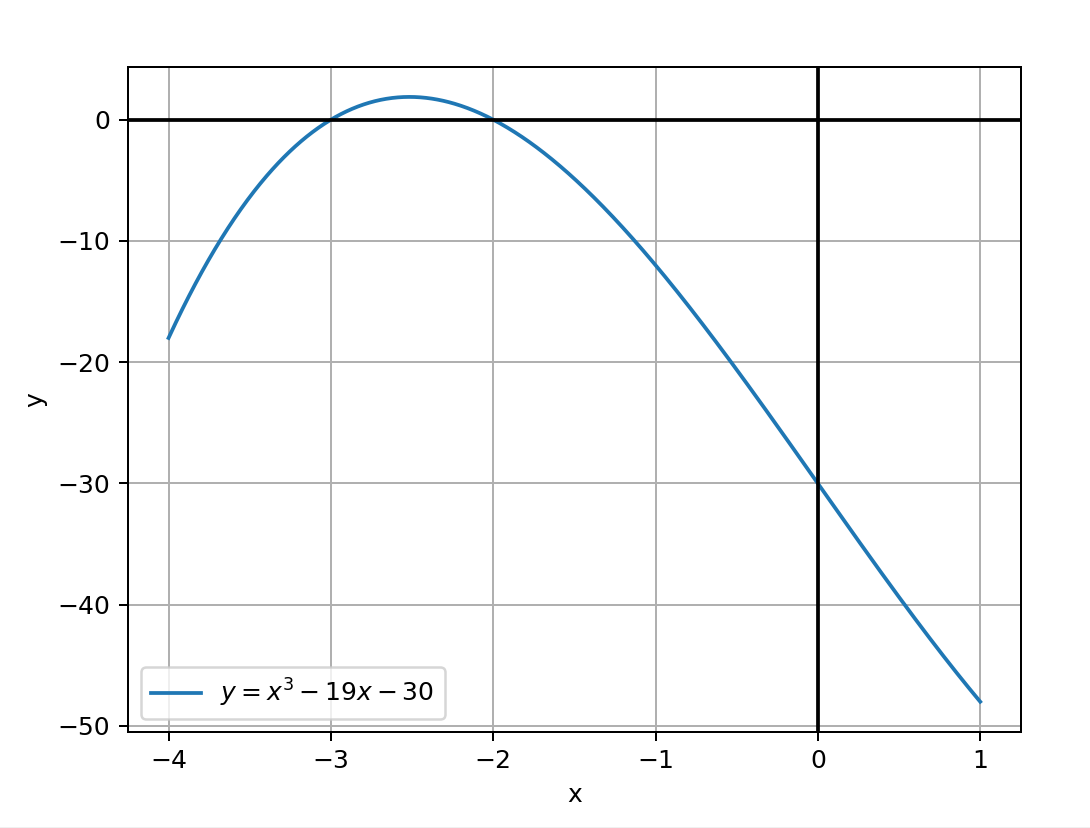
\includegraphics[width=0.5\textwidth]{Graph.png}
\label{graph}
   \end{itemize}
\end{document}
